
\section{Equacions de govern de la trajectòria}

\subsection{Sistema de referència}
Per tal d'estudiar el moviment i la trajectòria de qualssevol cos cal considerar uns eixos de coordenades. Per tal de poder aplicar la segona llei de Newton, és necessari que el sistema de coordenades considerat sigui inercial, dit d'una manera simple, un sistema de referència és inercial quan estan fixos o tenen moviment relatiu uniforme. És a dir, que la variació de moment lineal del sistema sigui igual a les forces reals sobre el sistema, de manera matemàtica, un sistema en el qual:
\begin{equation}
    \sum F_{\mathrm{reals}} = \frac{\dd \Vec{p}}{\dd t}
\end{equation}
Mentre que en la descripció no newtoniana d'un sistema de referencia NO inercial s'han d'afegir el terme de les forces fictícies $F_{\mathrm{fict}}$.
\begin{equation}
    \sum F_{\mathrm{reals}} + \sum F_{\mathrm{fict}}= \frac{\dd \Vec{p}}{\dd t}
\end{equation}

De sistemes de referència inercials es poden definir diferents. No obstant, per d'agilitzar els càlculs i simplificar les expressions, per aquest problema en particular es definiran els eixos horitzó local i el sitema de refe`rencia d'eixos vent [Figura \ref{fig:eixos_coordenades}]:

\begin{figure}[ht]
    \centering
    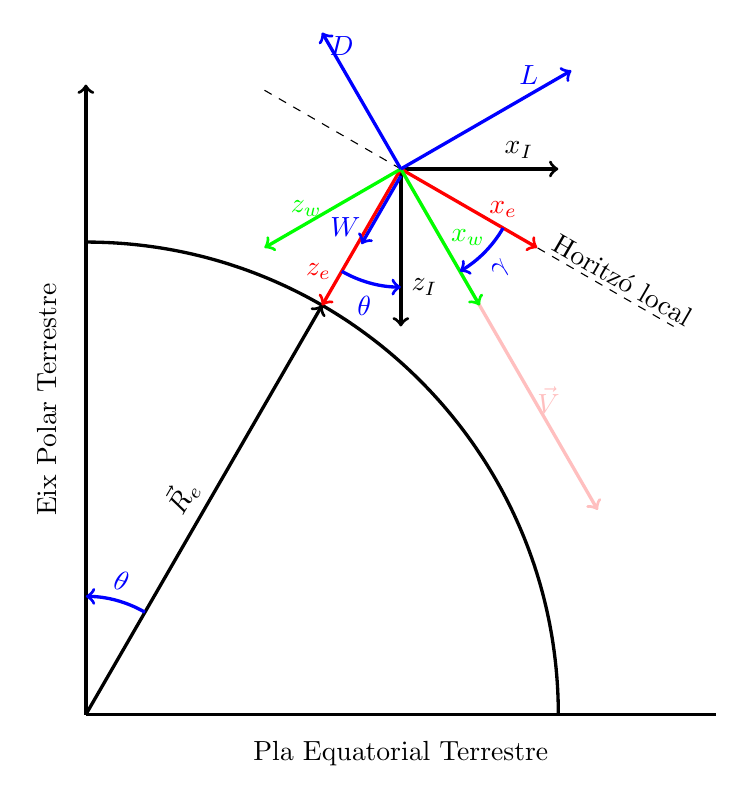
\begin{tikzpicture}
        % Definiciones
        \def\axislength{2}
        \def\measurelength{1.5}
        \def\windangle{60}
        \def\speedlength{5}
        % Ejeh tierra
        \draw[black, very thick] (0,0) -- (8,0);
        \node at (4,-0.5) {Pla Equatorial Terrestre};
        \draw[<-, black, very thick] (0,8) -- (0,0);
        \node[rotate=90] at (-0.5,4) {Eix Polar Terrestre};
        % Superficie terrestre
        \draw[black, very thick] (6,0) arc (0:90:6);
        %\draw[black, very thick] (0,0) -- ({8*cos(60)},{8*sin(60)});
        % Vector tierra
        \draw[<-, black, very thick] ({6*cos(60)}, {6*sin(60)}) -- node[midway, above, rotate=60]{$\vec{R}_e$} (0,0);
        \draw[<-, blue, very thick] (0,\measurelength) arc (90:60:\measurelength);
        \node[blue, rotate=-15] at ({(\measurelength+0.25)*cos(75)}, {(\measurelength+0.25)*sin(75)}) {$\theta$};
        % Vector velocidad
        \draw[<-, pink, very thick] ({8*cos(60)+\speedlength*cos(-\windangle)},{8*sin(60)+\speedlength*sin(-\windangle)}) --
                                    node[near start, above]{$\vec{V}$} ({8*cos(60)},{8*sin(60)});
        % Horizonte local
        \draw[black, dashed] ({8*cos(60)+2*cos(150)},{8*sin(60)+2*sin(150)}) -- ({8*cos(60)+4*cos(-30)},{8*sin(60)+4*sin(-30)});
        \node[black, rotate=-30, transform canvas={yshift=+6pt}] at ({8*cos(60)+3.25*cos(-30)},{8*sin(60)+3.25*sin(-30)}) {Horitzó local};
        % Ejeh inerciale
        \draw[<-, black, very thick] ({8*cos(60)+\axislength},{8*sin(60)}) -- node[near start, above]{$x_I$} ({8*cos(60)},{8*sin(60)});
        \draw[<-, black, very thick] ({8*cos(60)},{8*sin(60)-\axislength}) -- node[near start, right]{$z_I$} ({8*cos(60)},{8*sin(60)});
        % Ejeh tierra
        \draw[<-, red, very thick] ({8*cos(60)+\axislength*cos(-30)},{8*sin(60)+\axislength*sin(-30)}) -- 
                                    node[near start, above]{$x_e$} ({8*cos(60)},{8*sin(60)});
        \draw[<-, red, very thick] ({8*cos(60)+\axislength*cos(240)},{8*sin(60)+\axislength*sin(240)}) -- 
                                    node[near start, left]{$z_e$}({8*cos(60)},{8*sin(60)});
        % Ejeh uind
        \draw[<-, green, very thick] ({8*cos(60)+\axislength*cos(-\windangle)},{8*sin(60)+\axislength*sin(-\windangle)}) -- 
                                    node[midway, right]{$x_w$} ({8*cos(60)},{8*sin(60)});
        \draw[<-, green, very thick] ({8*cos(60)+\axislength*cos(270-\windangle)},{8*sin(60)+\axislength*sin(270-\windangle)}) -- 
                                    node[midway, left]{$z_w$}({8*cos(60)},{8*sin(60)});
        % Fuerzah de sustentación
        \draw[<-, blue, very thick] ({8*cos(60)+2.5*cos(90-\windangle)},{8*sin(60)+2.5*sin(90-\windangle)}) -- 
                                    node[near start, above]{$L$}({8*cos(60)},{8*sin(60)});
        % Fuerzah de resistencia
        \draw[<-, blue, very thick] ({8*cos(60)+2*cos(180-\windangle)},{8*sin(60)+2*sin(180-\windangle)}) -- node[near start, above]{$D$}({8*cos(60)},{8*sin(60)});
        % Fuerzah peso
        \draw[<-, blue, very thick, transform canvas={yshift=-2.5pt}] ({8*cos(60)+1*cos(240)},{8*sin(60)+1*sin(240)}) -- 
                                    node[near start, left]{$W$}({8*cos(60)},{8*sin(60)});
        % Cota angular 1
        \draw[<-, blue, very thick] ({8*cos(60)+\measurelength*cos(-\windangle)},{8*sin(60)+\measurelength*sin(-\windangle)}) 
                                    arc (-\windangle:-30:\measurelength);
        \node[blue, rotate=45] at ({8*cos(60)+(\measurelength+0.3)*cos(-45)},{8*sin(60)+(\measurelength+0.3)*sin(-45)}) {$\gamma$};
        % Cota angular 2
        \draw[<-, blue, very thick] ({8*cos(60)+\measurelength*cos(270)},{8*sin(60)+\measurelength*sin(270)})
                                    arc (270:240:\measurelength);
        \node[blue] at ({8*cos(60)+(\measurelength+0.3)*cos(255)},{8*sin(60)+(\measurelength+0.3)*sin(255)}) {$\theta$};
    \end{tikzpicture}
    \caption{Esquema del sistema de coordenades}
    \label{fig:eixos_coordenades}
\end{figure}

El sistema de referència d'eixos horitzó local es defineixen un pla horitzontal definida per $\hat{x}$ i $\hat{y}$ normalment en les quals apunten cap al nord i cap a l'est geogràfic, respectivament. Quedant per finalment, $\hat{z}$ definida cap al centre de la Terra.

Tanmateix, per l'estudi de les actuacions, els eixos de referència d'eixos vent són d'extrema utilitat doncs està lligat a la velocitat aerodinàmica instantània de l'avió on $\hat{z}$ està contingut en el pla de simetria i $hat{x}$ i $\hat{y}$ contindran les forces aerodinàmiques de sustentació $L$ i resistència aerodinàmica $D$.

\subsection{Equacions cinemàtiques i dinàmiques de la mecànica del vol}

Les equacions que governen la trajectòria de reentrada atmosfèrica es poden derivar de les equacions de la mecànica del vol. Les equacions cinemàtiques són \cite{gomez_tierno}:
\begin{empheq}[left = \empheqlbrace]{align}
    \dot{x} &= V \cos{\gamma'} \cos{\chi} \\
    \dot{y} &= V \cos{\gamma'} \sin{\chi} \\
    \dot{z} &= - \dot{h} = - V \sin{\gamma'}
\end{empheq}
I les equacions dinàmiques:
\begin{empheq}[left = \empheqlbrace]{align}
    &T \cos{\varepsilon} \cos{\nu} - D - m g \sin{\gamma'} - m \dot{V} = 0 \\
    &T \cos{\varepsilon} \sin{\nu} - F_y + m g \cos{\gamma'} \sin{\mu} + 
    m V \left(\dot{\gamma'} \sin{\mu} - \dot{\chi} \cos{\gamma'} \cos{\mu} \right) = 0 \\
  - &T \sin{\varepsilon} - L + m g \cos{\gamma'} \cos{\mu} + 
    m V \left( \dot{\gamma'} \cos{\mu} + \dot{\chi} \cos{\gamma'} \sin{\mu} \right) = 0
\end{empheq}
\noindent
Durant la reentrada no hi ha empenta, $T = 0$. Es considera que el vehicle es manté en un pla vertical, \ie, $\dot{y} = 0$, de mode que $\chi \in \left\{ 0, \pi \right\}$. Es suposa a més que el vol és simètric, $F_y = 0$ i $\mu = 0$. Prenent $\chi = 0$ i introduint aquestes simplificacions a les equacions anteriors, s'obté:
\begin{empheq}[left = \empheqlbrace]{align}
    \dot{x} &= V \cos{\gamma'} \\
    \dot{h} &= V \sin{\gamma'}
\end{empheq}
\begin{empheq}[left = \empheqlbrace]{align}
    &D + m g \sin{\gamma'} + m \dot{V} = 0 \\
    - &L + m g \cos{\gamma'} + m V \dot{\gamma'} = 0
\end{empheq}
\noindent
L'angle $\gamma'$ és l'angle ``de asiento'' de la velocitat, \ie, l'angle que forma l'eix $x_w$ amb el pla horitzontal. Atès que es tracta d'un descens, aquest és negatiu. Per simplificar les expressions, es pren l'angle $\gamma = - \gamma'$. Aleshores:
\begin{empheq}[left=\empheqlbrace]{align}
    \dot{x} &= V \cos{\gamma}       \label{eq:cinematica_x} \\
    \dot{h} &= - V \sin{\gamma}     \label{eq:cinematica_z}
\end{empheq}
\begin{empheq}[left=\empheqlbrace]{align}
    &D - m g \sin{\gamma} + m \dot{V} = 0           \label{eq:dinamica_x} \\
    - &L + m g \cos{\gamma} - m V \dot{\gamma} = 0  \label{eq:dinamica_z}
\end{empheq}
A partir d'aquest sistema de quatre equacions diferencials ordinàries es poden deduir les equacions de la reentrada sustentadora i de la reentrada balística.

\subsection{Equacions de govern de la reentrada sustentadora}

A partir de de l'equació \eqref{eq:dinamica_x}, s'obté la primera equació de la reentrada sustentadora:
\begin{equation*}
    \dot{V} = \frac{\dd V}{\dd t} = g \sin{\gamma} - \frac{D}{m} = g \sin{\gamma} - \frac{1}{2} \rho V^2 \frac{S C_D}{m} = 
    g \sin{\gamma} - Q g \frac{S C_D}{m g}
\end{equation*}
En el cas que el planeta on es fa la reentrada atmosfèrica sigui la Terra, es considera que aquesta comença al voltant dels $h_0 = 80 \ \kilo\meter$, on l'acceleració de la gravetat és $g(h_0) = 9.57825 \ \meter / \second^2$. Això representa una variació relativa respecte de l'acceleració de la gravetat a nivell del mar ($g_0 = 9.80665 \ \meter / \second^2$) del $2.32\%$. Es pot aproximar per tant $g \left( h_0 \right) \approx g_0$, i es té que
\begin{equation} \label{eq:derivada_V_t_lifting}
    \frac{\dd V}{\dd t} \approx g \sin{\gamma} - Q g \frac{S C_D}{m g_0} = 
    g \sin{\gamma} - \frac{Q}{\beta} g = g \left( \sin{\gamma} - \frac{Q}{\beta} \right)
\end{equation}

Partint de l'equació \eqref{eq:dinamica_z}, es dedueix la segona equació de la reentrada sustentadora:
\begin{align*}
    \dot{\gamma} &= \frac{\dd \gamma}{\dd t} = \frac{g \cos{\gamma} - \dfrac{L}{m}}{V} = 
    \frac{g \cos{\gamma} - \dfrac{1}{2} \rho V^2 \dfrac{S C_L}{m}}{V} = 
    \frac{g \cos{\gamma} - Q g \dfrac{S C_D}{m g} \dfrac{C_L}{C_D}}{V} \\
    &\approx \frac{g \cos{\gamma} - \dfrac{Q g}{\beta} \dfrac{C_L}{C_D}}{V} 
\end{align*}
Degut a que el vehicle de reentrada està girant, apareix una acceleració normal $V^2/ \left( R_p + h \right)$ de sentit contrari a l'acceleració de la gravetat $g$. Per tant, el primer terme del numerador s'ha de corregir restant aquesta acceleració. D'aquesta manera s'obté la segona equació:
\begin{equation} \label{eq:derivada_gamma_t_lifting}
    \frac{\dd \gamma}{\dd t} = \frac{\left( g - \dfrac{V^2}{R_p + h} \right) \cos{\gamma} - \dfrac{Q g}{\beta} \dfrac{C_L}{C_D}}{V}
\end{equation}

De l'equació \eqref{eq:cinematica_z}, es té directament la tercera equació de la reentrada sustentadora:
\begin{equation} \label{eq:derivada_h_t_lifting}
    \frac{\dd h}{\dd t} = - V \sin{\gamma}
\end{equation}
Sobre una circumferència de radi $R$, la longitud que abasta un arc d'angle angle $\theta$ és $L = R \theta$, amb $\theta$ en radians. En un instant de temps donat $t$, el vehicle es troba a una altitud $h$ sobre la superfície del planeta, per tant a una distància $R_p + h$ del centre del planeta. Durant un interval de temps $t + \dd t$ es pot considerar que les variables del descens no varien. Així, la distància horitzontal recorreguda és $\dd L = V \cos{\gamma} \, \dd t$ i l'angle abastat
\begin{equation*}
    \dd \theta = \frac{\dd L}{R_p + h} = \frac{V \cos{\gamma}}{R_p + h} \, \dd t
\end{equation*}
Conseqüentment, la projecció sobre la superfície del planeta és $\dd r = R_p \, \dd \theta$. Atès que $\dd t > 0$, es multiplica per $1 / \dd t$ a ambdues bandes de la igualtat i s'obté l'última equació de la reentrada sustentadora:
\begin{equation} \label{eq:derivada_r_t_lifting}
    \frac{\dd r}{\dd t} = \frac{R_p}{R_p + h} V \cos{\gamma}
\end{equation}

\subsection{Equacions de govern de la reentrada balística}

L'altitud del vehicle de reentrada és una funció contínua i derivable del temps, definida sobre un interval $\mathcal{I} = \left[ 0, t_\text{max} \right]$, \ie, $h \colon \mathcal{I} \to \mathcal{X} \subset \mathbb{R}$, on $\mathcal{X} = \left[ 0, h_\text{max} \right]$. En general, $h$ no és bijectiva, ja que en alguns casos de reentrada, el vehicle augmenta la seva altitud. No obstant, es poden trobar intervals $I \subseteq \mathcal{I}$ on la restricció de la funció a l'interval, $h \vert_{I} \colon I \to X \subseteq \mathcal{X}$, sigui bijectiva. Aquests intervals són aquells on $h$ és estrictament creixent o estrictament decreixent. En aquests casos la funció té una funció inversa local definida, \ie, $t \colon X \to I$, que és també contínua i derivable. En general, el vehicle no mantindrà alçada constant, per tant l'interval $\mathcal{I}$ es pot expressar com a unió dels intervals $I$ on $h$ és bijectiva, és a dir, $t$ es pot expressar com una funció a trossos. És sabut de l'anàlisi, que donada una funció $f$ amb inversa $f^{-1}$ en un punt que verifiqui les condicions prèvies, la derivada de $f^{-1}$ és la inversa de la derivada de $f$ \cite{zorich}. D'aquesta manera, a partir de l'equació \eqref{eq:derivada_h_t_lifting}, s'obté la primera equació de la reentrada balística,
\begin{equation} \label{eq:derivada_t_h_ballistic}
    \frac{\dd t}{\dd h} = \left( \frac{\dd h}{\dd t} \right)^{-1} = - \frac{1}{V \sin{\gamma}}
\end{equation}
Aplicant la regla de la cadena a l'expressió \eqref{eq:derivada_V_t_lifting} usant \eqref{eq:derivada_t_h_ballistic}, s'arriba a la segona equació de la reentrada balística:
\begin{equation} \label{eq:derivada_V_h_ballistic}
    \frac{\dd V}{\dd h} = \frac{\dd V}{\dd t} \frac{\dd t}{\dd h} = 
    \frac{ g \left( \dfrac{Q}{\beta} - \sin{\gamma} \right)}{V \sin{\gamma}}
\end{equation}
Durant la reentrada balística no hi ha sustentació, aleshores $C_L = 0$. Aplicant la regla de la cadena a l'equació \eqref{eq:derivada_gamma_t_lifting},
\begin{equation} \label{eq:derivada_gamma_h_ballistic}
    \frac{\dd \gamma}{\dd h} = \frac{\dd \gamma}{\dd t} \frac{\dd t}{\dd h} = 
    \frac{\left( \dfrac{V^2}{R_p + h} - g \right) \cos{\gamma}}{V^2 \sin{\gamma}}
\end{equation}
Novament, aplicant la regla de la cadena a l'equació \eqref{eq:derivada_r_t_lifting}, s'obté l'última equació de la reentrada balística:
\begin{equation} \label{eq:derivada_r_h_ballistic}
    \frac{\dd r}{\dd h} = \frac{\dd r}{\dd t} \frac{\dd t}{\dd h} = - \frac{R_p}{R_p + h} \frac{\cos{\gamma}}{\sin{\gamma}}
\end{equation}



